% =====================================================================
%  KARIOS CubeSat -- Verification Process
%  Detailed schematic block diagram (ECSS-E-ST-10 / MBSE)
%  Model strategy: EM -> EQM -> PFM   |   Review gates: full ECSS set
%
%  Compile:  pdflatex KARIOS_verification_block_diagram.tex
%  (standalone class crops the PDF to the diagram for figure inclusion)
% =====================================================================
\documentclass[border=14pt]{standalone}
\usepackage[T1]{fontenc}
\usepackage{helvet}
\renewcommand{\familydefault}{\sfdefault}
\usepackage{tikz}
\usetikzlibrary{positioning,arrows.meta,fit,backgrounds,calc}

% ---- palette ----
\definecolor{accent}{HTML}{2563A8}
\definecolor{ink}{HTML}{131B28}
\definecolor{ink3}{HTML}{6B7788}
\definecolor{line}{HTML}{C4CDD9}
\definecolor{surface}{HTML}{FFFFFF}
\definecolor{surface2}{HTML}{F1F4F9}
\definecolor{mtest}{HTML}{C9761F}
\definecolor{manalysis}{HTML}{2F74C0}
\definecolor{mreview}{HTML}{7C53A5}
\definecolor{minspect}{HTML}{1F8F86}
\definecolor{warn}{HTML}{C0632A}

\begin{document}
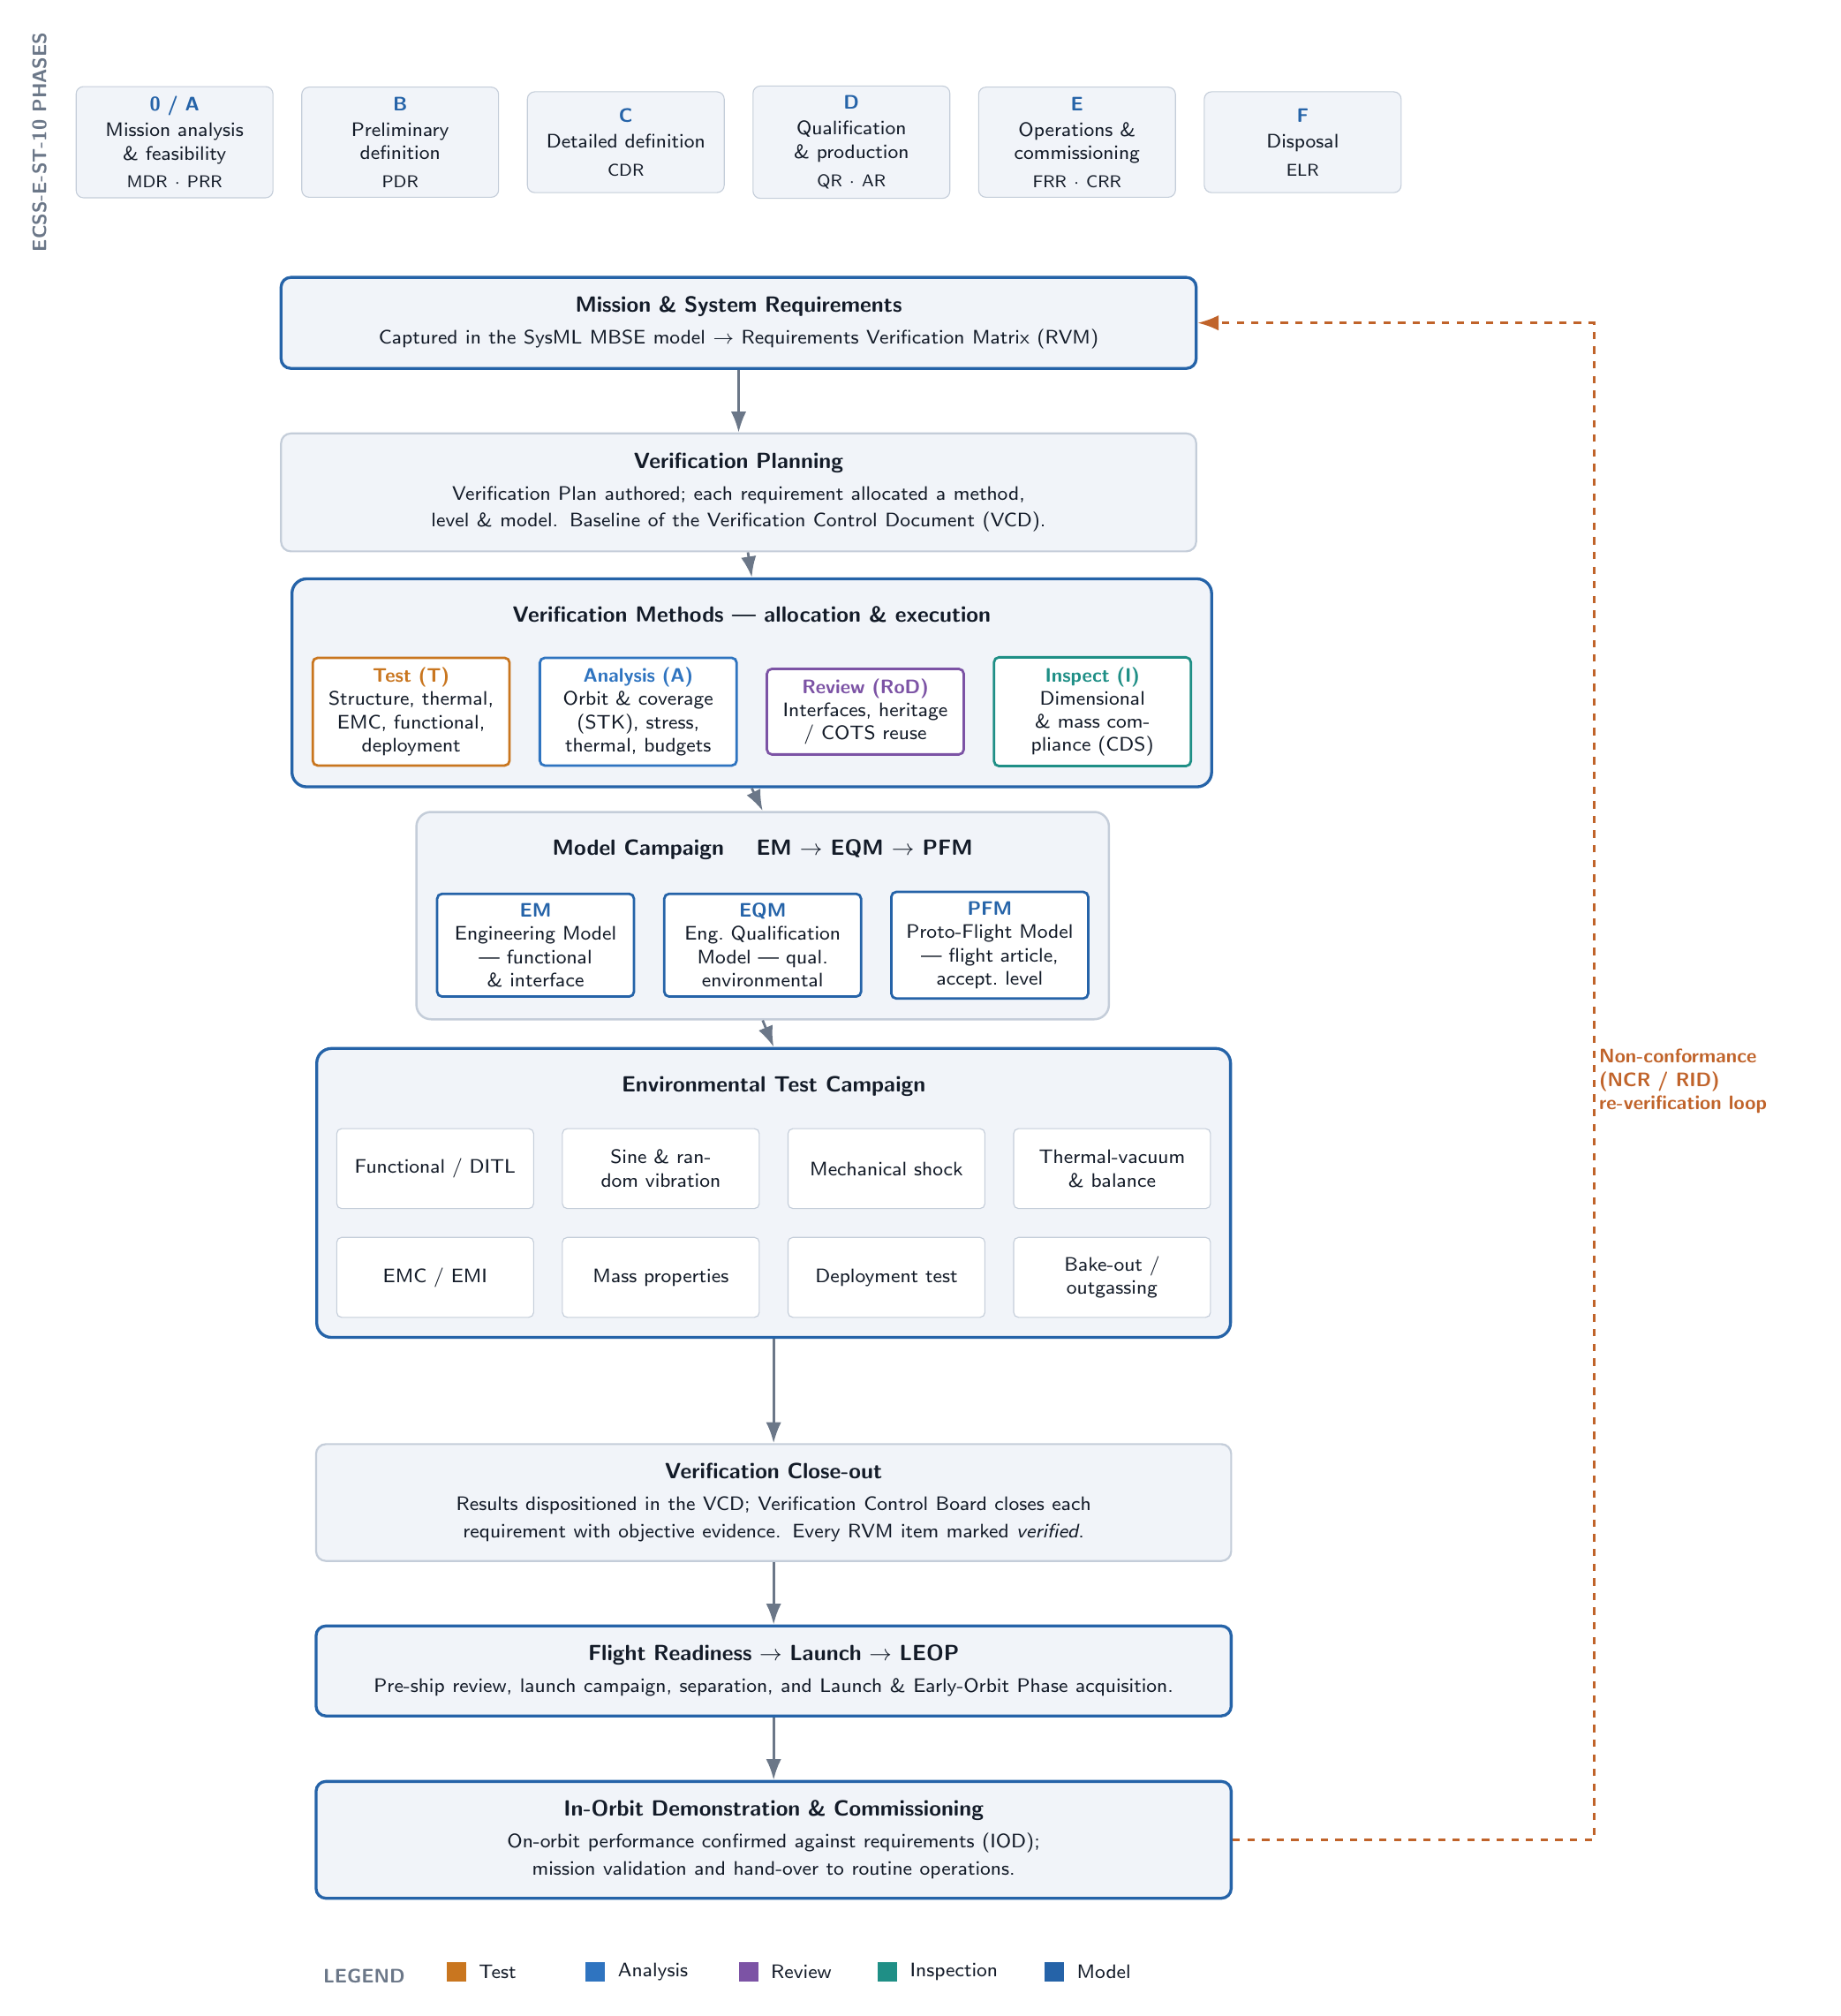
\begin{tikzpicture}[
  font=\small,
  every node/.style={text=ink},
  stage/.style={draw=line, line width=0.8pt, rounded corners=4pt, fill=surface2,
                text width=12.6cm, align=center, inner sep=8pt},
  keystage/.style={stage, draw=accent, line width=1.2pt},
  stitle/.style={font=\bfseries},
  arrow/.style={-{Latex[length=3mm,width=2.2mm]}, line width=1pt, draw=ink3},
  phase/.style={draw=line, rounded corners=3pt, fill=surface2, text width=2.55cm,
                align=center, inner sep=4pt, minimum height=1.45cm, font=\footnotesize},
  gtitle/.style={font=\bfseries\small, text=ink},
  chip/.style={draw=line, rounded corners=2pt, fill=surface, text width=2.55cm,
               align=center, inner sep=4pt, minimum height=1.15cm, font=\footnotesize},
  chipT/.style={chip, draw=mtest, line width=1pt},
  chipA/.style={chip, draw=manalysis, line width=1pt},
  chipR/.style={chip, draw=mreview, line width=1pt},
  chipI/.style={chip, draw=minspect, line width=1pt},
  chipM/.style={chip, draw=accent, line width=1pt},
  groupbox/.style={draw=line, line width=0.9pt, rounded corners=6pt, fill=surface2, inner sep=8pt},
  keygroupbox/.style={groupbox, draw=accent, line width=1.2pt},
]

% ---------- ECSS phase timeline ----------
\node[phase] (ph0) {\textbf{\textcolor{accent}{0 / A}}\\[1pt]Mission analysis \& feasibility\\[2pt]{\scriptsize MDR $\cdot$ PRR}};
\node[phase, right=4mm of ph0] (phB) {\textbf{\textcolor{accent}{B}}\\[1pt]Preliminary definition\\[2pt]{\scriptsize PDR}};
\node[phase, right=4mm of phB] (phC) {\textbf{\textcolor{accent}{C}}\\[1pt]Detailed definition\\[2pt]{\scriptsize CDR}};
\node[phase, right=4mm of phC] (phD) {\textbf{\textcolor{accent}{D}}\\[1pt]Qualification \& production\\[2pt]{\scriptsize QR $\cdot$ AR}};
\node[phase, right=4mm of phD] (phE) {\textbf{\textcolor{accent}{E}}\\[1pt]Operations \& commissioning\\[2pt]{\scriptsize FRR $\cdot$ CRR}};
\node[phase, right=4mm of phE] (phF) {\textbf{\textcolor{accent}{F}}\\[1pt]Disposal\\[2pt]{\scriptsize ELR}};

\node[font=\bfseries\footnotesize, text=ink3, left=3mm of ph0, rotate=90, anchor=south] {ECSS-E-ST-10 PHASES};

% center axis under the phase strip
\coordinate (mid) at ($(phC.south)!0.5!(phD.south)$);

% ---------- main vertical flow ----------
\node[keystage, below=1.15cm of mid] (req)
   {{\bfseries{}Mission \& System Requirements}\\[2pt]
    {\footnotesize Captured in the SysML MBSE model $\rightarrow$ Requirements Verification Matrix (RVM)}};

\node[stage, below=0.9cm of req] (plan)
   {{\bfseries{}Verification Planning}\\[2pt]
    {\footnotesize Verification Plan authored; each requirement allocated a method, level \& model. Baseline of the Verification Control Document (VCD).}};

% ----- methods group -----
\node[chipT, below=1.5cm of plan, xshift=-4.71cm] (mT)
   {\textbf{\textcolor{mtest}{Test (T)}}\\ Structure, thermal, EMC, functional, deployment};
\node[chipA, right=4mm of mT] (mA)
   {\textbf{\textcolor{manalysis}{Analysis (A)}}\\ Orbit \& coverage (STK), stress, thermal, budgets};
\node[chipR, right=4mm of mA] (mR)
   {\textbf{\textcolor{mreview}{Review (RoD)}}\\ Interfaces, heritage / COTS reuse};
\node[chipI, right=4mm of mR] (mI)
   {\textbf{\textcolor{minspect}{Inspect (I)}}\\ Dimensional \& mass compliance (CDS)};
\node[gtitle] (mttl) at ([yshift=6mm]$(mT.north)!0.5!(mI.north)$) {Verification Methods --- allocation \& execution};
\begin{scope}[on background layer]
  \node[keygroupbox, fit=(mttl)(mT)(mI)] (methodsbox) {};
\end{scope}

% ----- model campaign group -----
\node[chipM, below=1.5cm of methodsbox.south, xshift=-3.11cm] (cEM)
   {\textbf{\textcolor{accent}{EM}}\\ Engineering Model --- functional \& interface};
\node[chipM, right=4mm of cEM] (cEQM)
   {\textbf{\textcolor{accent}{EQM}}\\ Eng.\ Qualification Model --- qual.\ environmental};
\node[chipM, right=4mm of cEQM] (cPFM)
   {\textbf{\textcolor{accent}{PFM}}\\ Proto-Flight Model --- flight article, accept.\ level};
\node[gtitle] (cttl) at ([yshift=6mm]$(cEM.north)!0.5!(cPFM.north)$) {Model Campaign \quad EM $\rightarrow$ EQM $\rightarrow$ PFM};
\begin{scope}[on background layer]
  \node[groupbox, fit=(cttl)(cEM)(cPFM)] (modelsbox) {};
\end{scope}

% ----- environmental test campaign group (2 x 4) -----
\node[chip, below=1.55cm of modelsbox.south, xshift=-4.71cm] (e1) {Functional / DITL};
\node[chip, right=4mm of e1] (e2) {Sine \& random vibration};
\node[chip, right=4mm of e2] (e3) {Mechanical shock};
\node[chip, right=4mm of e3] (e4) {Thermal-vacuum \& balance};
\node[chip, below=4mm of e1] (e5) {EMC / EMI};
\node[chip, right=4mm of e5] (e6) {Mass properties};
\node[chip, right=4mm of e6] (e7) {Deployment test};
\node[chip, right=4mm of e7] (e8) {Bake-out / outgassing};
\node[gtitle] (ettl) at ([yshift=6mm]$(e1.north)!0.5!(e4.north)$) {Environmental Test Campaign};
\begin{scope}[on background layer]
  \node[keygroupbox, fit=(ettl)(e1)(e4)(e5)(e8)] (envbox) {};
\end{scope}

\node[stage, below=1.5cm of envbox.south] (close)
   {{\bfseries{}Verification Close-out}\\[2pt]
    {\footnotesize Results dispositioned in the VCD; Verification Control Board closes each requirement with objective evidence. Every RVM item marked \emph{verified}.}};

\node[keystage, below=0.9cm of close] (flight)
   {{\bfseries{}Flight Readiness $\rightarrow$ Launch $\rightarrow$ LEOP}\\[2pt]
    {\footnotesize Pre-ship review, launch campaign, separation, and Launch \& Early-Orbit Phase acquisition.}};

\node[keystage, below=0.9cm of flight] (iod)
   {{\bfseries{}In-Orbit Demonstration \& Commissioning}\\[2pt]
    {\footnotesize On-orbit performance confirmed against requirements (IOD); mission validation and hand-over to routine operations.}};

% ---------- connecting arrows ----------
\draw[arrow] (req) -- (plan);
\draw[arrow] (plan) -- (methodsbox.north);
\draw[arrow] (methodsbox.south) -- (modelsbox.north);
\draw[arrow] (modelsbox.south) -- (envbox.north);
\draw[arrow] (envbox.south) -- (close.north);
\draw[arrow] (close) -- (flight);
\draw[arrow] (flight) -- (iod);

% ---------- feedback loop (orthogonal: right -> up -> left) ----------
\draw[arrow, draw=warn, dashed]
   (iod.east) -- ++(5.2,0) |- (req.east);
\node[anchor=west, text width=3cm, align=left, font=\footnotesize\bfseries, text=warn]
   at ([xshift=5.4cm]$(iod.east)!0.5!(req.east)$)
   {Non-conformance\\ (NCR / RID)\\ re-verification loop};

% ---------- legend ----------
\begin{scope}[shift={($(iod.south west)+(0,-1.1cm)$)}]
  \node[anchor=west, font=\footnotesize\bfseries, text=ink3] at (0,0) {LEGEND};
  \foreach \x/\c/\t in {1.9/mtest/Test, 3.9/manalysis/Analysis, 6.1/mreview/Review, 8.1/minspect/Inspection, 10.5/accent/Model} {
     \fill[\c] (\x,-0.08) rectangle ++(0.28,0.28);
     \node[anchor=west, font=\footnotesize, text=ink] at (\x+0.34,0.06) {\t};
  }
\end{scope}

\end{tikzpicture}
\end{document}
